\chapter{Исследовательская часть}

\section{Технические характеристики}

Технические характеристики устройства, на котором выполнялись замеры по времени, представлены далее.

\begin{enumerate}
	\item Процессор	Intel(R) Core(TM) i7-9750H CPU @ 2.60GHz, 2592 МГц, ядер: 6, логических процессоров: 12;
	\item Оперативная память: 16 ГБайт;
	\item Операционная система: Майкрософт Windows 10 Pro \cite{windows};
	\item Использованная подсистема: WSL2 \cite{WSL2}.
\end{enumerate}

При замерах времени ноутбук был включен в сеть электропитания и был нагружен только системными приложениями.

\section{Демонстрация работы программы}

На рисунке \ref{img:demonstration} представлена демонстрация работы разработанного программного обеспечения, 
показаны результаты вычислений расстояний Дамерау--Левенштейна и Левенштейна между словами <<fds>>,<<asd>>, заметим
что в случае поднятого флага вывода матриц происходит вывод матриц, использованных в расчетах.
\clearpage
\begin{figure}[H]
	\centering
	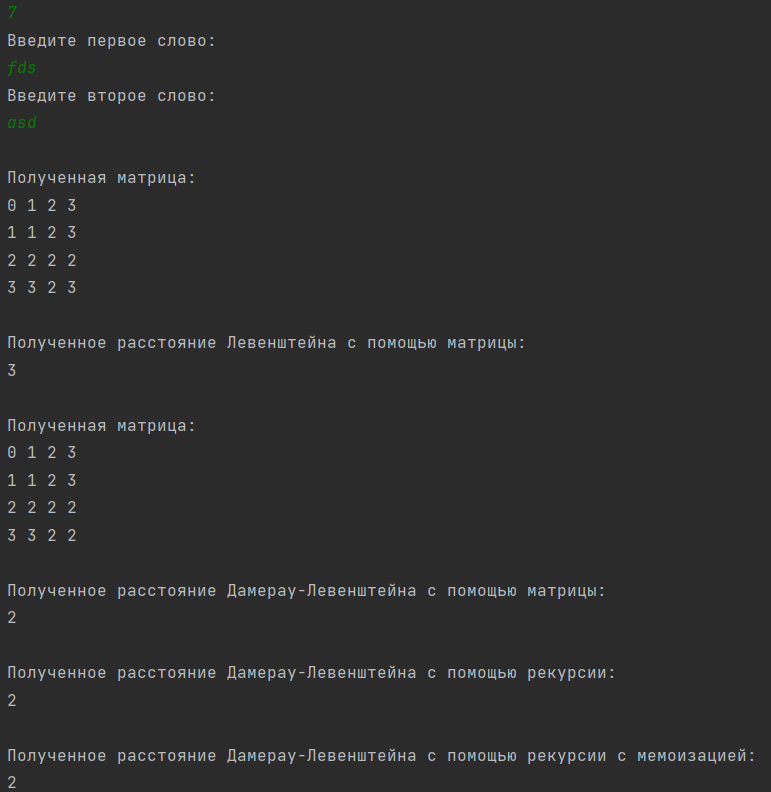
\includegraphics[height=0.7\textheight]{../img/programm_work.png}
	\caption{Демонстрация работы программы}
	\label{img:demonstration}
\end{figure}

\clearpage

\section{Временные характеристики}

Результаты исследования замеров по времени приведены в таблице \ref{t:timings}.
Введем следующие обозначения для чтения таблиц:
\begin{enumerate}
	\item n --- длина анализируемых строк;
	\item ДМ --- реализация алгоритма поиска расстояния Дамерау---Левенштейна с использованием матрицы;
	\item ДР --- рекурсивная реализация алгоритма поиска расстояния Дамерау---Левенштейна;
	\item ДРМ ---  рекурсивная реализация алгоритма поиска расстояния Дамерау---Левенштейна с использованием мемоизации;
	\item ЛМ --- реализация алгоритма поиска расстояния Левенштейна с использованием матрицы.
\end{enumerate}

Заметим, что некоторые поля в данной таблице
имеют значение <<$\sim$>>, это обусловлено тем, что дальнейший расчет значений столбца <<ДР>> окажется слишком
долгим, полученных данных достаточно для проведения исследования.

Замеры проводились на одинаковых длин строк от 0 до 1000 с различным шагом, для получения достоверных результатов замеры 
времени для каждой пары строк проводились 100 раз, после чего усреднялись. Все результаты вычислений приведены в миллисекундах.




\begin{table}[!ht]
	\centering
	\caption{Полученная таблица замеров по времени различных реализаций алгоритмов поиска редакционных расстояний}
	\begin{tabular}{|c|c|c|c|c|}
	\hline
	n  & ДМ, мс & ДР, мс & ДРМ, мс & ЛМ, мс \\
	\hline
		0    & 0.00118            & 0.00106               & 0.00109                     & 0.00106                \\ \hline
		3    & 0.00172            & 0.00219               & 0.00203                     & 0.00162                \\ \hline
		6    & 0.00308            & 0.12611               & 0.00388                     & 0.00284                \\ \hline
		9    & 0.0039             & 13.261                & 0.00534                     & 0.00338                \\ \hline
		12   & 0.00592            & 2489.9                & 0.00845                     & 0.00565                \\ \hline
		15   & 0.0082             & $\sim$                & 0.0115                      & 0.00751                \\ \hline
		18   & 0.01115            & $\sim$                & 0.01612                     & 0.01125                \\ \hline
		21   & 0.01484            & $\sim$                & 0.02665                     & 0.01379                \\ \hline
		24   & 0.02121            & $\sim$                & 0.0322                      & 0.02028                \\ \hline
		27   & 0.02374            & $\sim$                & 0.03873                     & 0.02401                \\ \hline
		30   & 0.02922            & $\sim$                & 0.04384                     & 0.02638                \\ \hline
		33   & 0.03526            & $\sim$                & 0.05304                     & 0.03204                \\ \hline
		36   & 0.04217            & $\sim$                & 0.06269                     & 0.03945                \\ \hline
		39   & 0.05094            & $\sim$                & 0.07313                     & 0.0461                 \\ \hline
		42   & 0.05838            & $\sim$                & 0.08418                     & 0.05092                \\ \hline
		45   & 0.06476            & $\sim$                & 0.09546                     & 0.06141                \\ \hline
		48   & 0.07404            & $\sim$                & 0.11081                     & 0.06931                \\ \hline
		51   & 0.08159            & $\sim$                & 0.12869                     & 0.07557                \\ \hline
		54   & 0.09406            & $\sim$                & 0.14051                     & 0.0834                 \\ \hline
		57   & 0.10324            & $\sim$                & 0.15499                     & 0.09519                \\ \hline
		60   & 0.11433            & $\sim$                & 0.16834                     & 0.10287                \\ \hline
		100  & 0.35718            & $\sim$                & 0.52154                     & 0.3144                 \\ \hline
		200  & 1.4173             & $\sim$                & 2.1709                      & 1.2841                 \\ \hline
		250  & 2.1346             & $\sim$                &  3.2308                      & 1.932                  \\ \hline
		300  & 3.1116             & $\sim$                & 4.5585                      & 2.7687                 \\ \hline
		350  & 4.2326             & $\sim$                & 6.2579                      & 3.765                  \\ \hline
		400  & 5.6911             & $\sim$                & 8.496                       & 5.1047                 \\ \hline
		450  & 7.0994             & $\sim$                & 10.566                      & 6.3133                 \\ \hline
		500  & 13.026             & $\sim$                & 18.581                      & 10.773                 \\ \hline
		550  & 12.199             & $\sim$                & 18.843                      & 11.238                 \\ \hline
		600  & 12.535             & $\sim$                & 19.627                      & 11.554                 \\ \hline
		650  & 15.848             & $\sim$                & 24.023                      & 14.052                 \\ \hline
		700  & 16.969             & $\sim$                & 25.572                      & 15.589                 \\ \hline
		750  & 19.061             & $\sim$                & 28.137                      & 17.093                 \\ \hline
		800  & 21.755             & $\sim$                & 32.658                      & 19.87                  \\ \hline
		850  & 24.98              & $\sim$                & 37.308                      & 22.387                 \\ \hline
		900  & 27.001             & $\sim$                & 41.447                      & 24.493                 \\ \hline
		950  & 29.422             & $\sim$                & 44.218                      & 26.874                 \\ \hline
		1000 & 32.658             & $\sim$                & 49.082                      & 29.756                \\ \hline
	\end{tabular}
	\label{t:timings}
\end{table}





 Приведенные  графики \ref{plt:time_matrix_cmp}--\ref{plt:time_mat_rec_cmp}  получены при 
помощи анализа данных таблицы \ref{t:timings}.

\begin{figure}[H]
	\centering
	\includesvg[height=0.3\textheight]{../img/matrixCmp.svg}
	\caption{Сравнение по времени нерекурсивных реализаций алгоритмов поиска расстояний Левенштейна и Дамерау---Левенштейна}
	\label{plt:time_matrix_cmp}
\end{figure}




\begin{figure}[H]
	\centering
	\includesvg[height=0.3\textheight]{../img/recCmp.svg}
	\caption{Сравнение по времени реализации рекурсивного поиска расстояния Дамерау---Левенштейна с мемоизацией и без, при использовании логарифмической шкалы}
	\label{plt:time_rec_cmp}
\end{figure}


\begin{figure}[H]
	\centering
	\includesvg[height=0.3\textheight]{../img/matRecCmp.svg}
	\caption{Сравнение по времени реализации рекурсивного поиска расстояния Дамерау---Левенштейна с  мемоизацией, с поиском
	расстояния с использоавнием матрицы}
	\label{plt:time_mat_rec_cmp}
\end{figure}


\section{Характеристики по памяти}

Введем следующие обозначения:
\begin{enumerate}
	\item $size_{1}$ --- длина строки $S_{1}$;
	\item $size_{2}$ --- длина строки $S_{2}$;
	\item $sizeof$ --- функция вычисляющая размер в байтах;
	\item $wstring$ --- строковый тип;
	\item $wstring\&$ --- указатель на строковый тип;
	\item $matrix\&$ --- указатель на матрицу;
	\item $int$ --- целочисленный тип;
	\item $size\_t$ --- беззнаковый целочисленный тип.
\end{enumerate}

Максимальная глубина стека вызовов при рекурсивной реализации нахождения расстояния Дамерау---Левенштейна равна сумме входящих строк,
так как дерево рекурсии будет расти пока длина хотя бы одной строки не будет равна 0. Таким образом при рекурсивном поиске данного расстояния затраченная память
будет рассчитываться  аналогично примеру (\ref{eq:dl_rec_memory}).
\begin{equation}
	\label{eq:dl_rec_memory}
	(n + m) \cdot (2 \cdot sizeof(wstring\&) + sizeof(int) + 6 \cdot sizeof(size\_t)) + 2 \cdot sizeof(wstring),
\end{equation}
где:
\begin{itemize}
	\item $2 \cdot sizeof(string)$ --- хранение двух строк;
	\item $2 \cdot sizeof(int)$ --- хранение размеров рассматриваемых подстрок;
	\item $2 \cdot sizeof(string\&)$ --- хранение указателей на строки;
	\item $6 \cdot sizeof(size\_t)$ --- вспомогательные переменные;
	\item $sizeof(int)$ --- адрес возврата.
\end{itemize}

Заметим, что в данном случае считается, что в типе $string$ хранятся все необходимые данные для задания строки(т.е. $size + 1$ символ).

Для рекурсивного алгоритма c кешированием поиска расстояния Дамерау---Левенштейна будет теоретически схож с расчетом в формуле (\ref{eq:dl_rec_memory}),
но также учитывается матрица, соответственно, максимальный расход памяти равен:
\begin{equation}
	\label{eq:dl_hash_memory}
    \small
	\begin{aligned}
		(n + m) \cdot (2 \cdot sizeof(string\&) + sizeof(int)+\\ +sizeof(matrix\&) + 6 \cdot sizeof(size\_t))+ \\
        + (2 \cdot sizeof(string) + sizeof(matrix)).
	\end{aligned}
\end{equation}

Затраты памяти на хранение матрицы описаны в  (\ref{eq:matrix_mem}).
\begin{equation}
	\label{eq:matrix_mem}
    \begin{aligned}
	sizeof(matrix) = sizeof(int) \cdot (n+1) \cdot (m + 1)+  \\
    + sizeof(int) \cdot 2 + sizeof(int\&) \cdot (n + 1) + sizeof(int\&\&).
    \end{aligned}
\end{equation}
В данном случае считается, что:
\begin{itemize}
	\item $sizeof(int) \cdot (n+1) \cdot (m + 1)$ --- хранение данных матрицы;
	\item $sizeof(int) \cdot 2$ --- хранение размеров матрицы;
	\item $sizeof(int\&) \cdot (n + 1)$ --- хранение строк матрицы;
	\item $sizeof(int\&\&)$ --- хранение указателя на матрицу.
\end{itemize}


Использование памяти при итеративной реализации алгоритма поиска расстояния Левенштейна  равно:
\begin{equation}
	\label{eq:lev_mtr_memory}
	\begin{aligned}
		sizeof(matrix) + sizeof(matrix\&) + 2 \cdot sizeof(wstring\&)+\\
        + 2 \cdot sizeof(wstring) + sizeof(int) + 3 \cdot sizeof(int),
	\end{aligned}
\end{equation}
где:
\begin{itemize}
	\item $sizeof(matrix) + sizeof(matrix\&)$ --- хранение матрицы и ее указателя в кадре стека;
	\item $2 \cdot sizeof(wstring) + 2 \cdot sizeof(wstring)$ --- хранение строк и их указателей в кадре стека;
	\item $(n + 1) \cdot (m + 1) \cdot size(int)$ --- хранение матрицы;
	\item $3 \cdot sizeof(int)$ --- вспомогательные переменные;
	\item $sizeof(int)$ --- адрес возврата.
\end{itemize}

Использование памяти при итеративной реализации алгоритма поиска расстояния Дамерау---Левенштейна аналогично приведенному
в (\ref{eq:lev_mtr_memory}).

По приведенным формулам затрат по памяти в программе были написаны соответствующие функции для подсчета расходуемой памяти, результаты расчетов, которые представлены в таблице \ref{t:memory}, где размеры строк находятся в диапазоне от 10 до 200 с шагом 10, результаты расчетов представлены в байтах.

\clearpage

\begin{table}[!ht]
    \centering
    \caption{Полученная таблица замеров по памяти различных реализаций алгоритмов поиска редакционных расстояний}
    \begin{tabular}{|c|c|c|c|c|}
    \hline
        n & ДМ, байт & ДР, байт & ДРМ, байт & ЛМ, байт \\ \hline
        0 & 200 & 64 & 132 & 200 \\ \hline
        10 & 760 & 2464 & 3652 & 760 \\ \hline
        20 & 2120 & 4864 & 7972 & 2120 \\ \hline
        30 & 4280 & 7264 & 13092 & 4280 \\ \hline
        40 & 7240 & 9664 & 19012 & 7240 \\ \hline
        50 & 11000 & 12064 & 25732 & 11000 \\ \hline
        60 & 15560 & 14464 & 33252 & 15560 \\ \hline
        70 & 20920 & 16864 & 41572 & 20920 \\ \hline
        80 & 27080 & 19264 & 50692 & 27080 \\ \hline
        90 & 34040 & 21664 & 60612 & 34040 \\ \hline
        100 & 41800 & 24064 & 71332 & 41800 \\ \hline
        110 & 50360 & 26464 & 82852 & 50360 \\ \hline
        120 & 59720 & 28864 & 95172 & 59720 \\ \hline
        130 & 69880 & 31264 & 108292 & 69880 \\ \hline
        140 & 80840 & 33664 & 122212 & 80840 \\ \hline
        150 & 92600 & 36064 & 136932 & 92600 \\ \hline
        160 & 105160 & 38464 & 152452 & 105160 \\ \hline
        170 & 118520 & 40864 & 168772 & 118520 \\ \hline
        180 & 132680 & 43264 & 185892 & 132680 \\ \hline
        190 & 147640 & 45664 & 203812 & 147640 \\ \hline
        200 & 163400 & 48064 & 222532 & 163400 \\ \hline
    \end{tabular}
     \label{t:memory}
\end{table}



\begin{figure}[H]
	\centering
	\includesvg[height=0.3\textheight]{../img/matRecCmpMem.svg}
	\caption{Сравнение по памяти алгоритмов поиска расстояния Левенштейна и Дамерау---Левенштейна --- итеративной и рекурсивной реализации}
	\label{plt:memory_mat_rec}
\end{figure}



\begin{figure}[H]
	\centering
	\includesvg[height=0.3\textheight]{../img/recCmpMem.svg}
	\caption{Сравнение по памяти алгоритмов поиска расстояния Дамерау---Левенштейна --- рекурсивной реализации с мемоизацией и без}
	\label{plt:memory_rec}
\end{figure}

\clearpage

\section{Результаты анализа различных реализаций}

\subsection{Сравнение по времени исполнения}
Имеет смысл сравнить поиск расстояний Левенштейна и Дамерау---Левенштейна при использовании матрицы, используя рисунок
\ref{plt:time_matrix_cmp}. Заметим, что при использовании
алгоритма поиска расстояния Дамерау---Левенштейна, при рассмотрении слов длины больше 50 затрачивается в 1.1 раз больше времени, чем 
при использовании алгоритма Левенштейна. Данная закономерность обусловлена дополнительной операцией обмена символов, которую 
необходимо учитывать при поиске расстояния Дамерау---Левенштейна.

Также необходимо сравнить реализации рекурсивного поиска расстояния Дамерау---Левенштейна с мемоизацией и без, полученный график приведен
на картинке \ref{plt:time_rec_cmp}. Заметим, что рекурсия с мемоизацией, за счет сохранения информации о уже рассчитанных расстояниях подстрок
показала себя в 29455 раз лучше, чем рекурсия без мемоизации.
При использовании рекурсии без мемоизации дерево рекурсии будет расти пока длина двух строк не будет равна 0. При спуске по дереву рекурсии каждый раз необходимо будет рассматривать 4 случая (обмен местами пар букв слова, вставка символа, удаление символа, замена символа) с построением полной ветви дерева рекурсии пока длина одного из слов не станет 0. При использовании мемоизации
рассчитанные значения сохраняются, благодаря чему можно не рассматривать уже полученные расстояния и брать необходимое значение из сохраненных, что дает значительный выигрыш в скорости получения требуемых значений.

Стоит отметить, что при сравнении реализации рекурсивного поиска расстояния Дамерау---Левенштейна с  мемоизацией и поиска
с использованием матрицы (графики замеров представлены на рисунке \ref{plt:time_mat_rec_cmp}), реализация с использованием матрицы показала себя более эффективной
по времени, затратив в 1.47 раз меньше миллисекунд. 
Наименее затратным по времени является итеративная реализация  алгоритма нахождения расстояния Левенштейна.

\subsection{Сравнение затраченной памяти}

Проанализировав таблицу \ref{t:memory}, можно сделать вывод, что по расходу памяти итеративные алгоритмы 
проигрывают рекурсивным: максимальный размер используемой памяти в итеративном растет как произведение длин строк,
в то время как у рекурсивного алгоритма --- как сумма длин строк.
Также стоит отметить, что при малых длинах слов рекурсивные алгоритмы уступают итеративным, это обусловлено большим 
количеством вспомогательных переменных в реализации рекурсивного алгоритма. Наиболее эффективным по памяти является рекурсивная реализация алгоритма поиска расстояния Дамерау---Левенштейна.


Рекурсивная реализация алгоритма поиска расстояния Дамерау---Левенштейна будет более затратной по времени по сравнению с итеративной реализацией алгоритма поиска расстояния Дамерау---Левенштейна, но менее затратным по памяти по отношению к итеративному алгоритму Дамерау---Левенштейна.
